%%%%%%%%%%%%%%%%%%%%%%%%%%%%%%%%%%%%%%%%%%%%%%%%%%%%%%%%%%%%%%%%%%%%%%%%%%%%%%
% Projet de PdP :  logiciel de génération de playlists musicales à partir
% d’une base de données contenant les descripteurs audio et métadonnées
% décrivant des morceaux de musiques
% Auteurs : Baptiste Fumaroli, Jean Pecqueur, Thomas Pizon et Lucas Vauzelle
% Date : février 2014
%%%%%%%%%%%%%%%%%%%%%%%%%%%%%%%%%%%%%%%%%%%%%%%%%%%%%%%%%%%%%%%%%%%%%%%%%%%%%%

\documentclass[11pt,a4paper]{article}

\usepackage[francais]{babel}
\usepackage[T1]{fontenc}
\usepackage[utf8]{inputenc}
\usepackage[left=3.5cm, right=3.5cm,top=3cm, bottom=3cm]{geometry}
\usepackage{titling}
\usepackage{fancyhdr}
\usepackage{graphicx}
\usepackage{subfig}
\usepackage{url}
\usepackage{amsmath}

\pagestyle{fancyplain}

\setlength{\droptitle}{-2cm}
\setlength{\headheight}{26pt}

\fancyhead[L,C,R]{}
\fancyhead[L]{Baptiste Fumaroli, Jean Pecqueur\\Thomas Pizon, Lucas Vauzelle}
\fancyhead[R]{\today \\Projet de Programmation}

\title{
\vspace{\fill}
\Huge{
Projet de Programmation:\\Générateur de playlists musicales
\\-\\
Analyse des besoins
}
\vspace{\fill}
}

\author{}
\date{}

\begin{document}

\maketitle
\newpage

\tableofcontents
\newpage

\section*{Introduction}

Dans le cadre de l’UE «~Projet de programmation~» du semestre~8 de Master~1
Informatique à l’Université de Bordeaux, Pierre Hanna, enseignant chercheur au
Laboratoire Bordelais de Recherche en Informatique nous a soumis un sujet en
rapport avec son domaine de recherche, l’informatique musicale.

\subsection*{Objectifs}

Le client dispose d’une base de données remplie suivant des critères bien précis
qui permettent de décrire et d'identifier des morceaux de musique. Notre objectif
est d’utiliser cette base de données comme outil pour créer un générateur de
playlists musicales, c’est à dire un enchaînement de morceaux destinés à être
joués successivement. L’utilisateur du logiciel aura la possibilité d’entrer des
paramètres permettant d’influencer la création de la playlist. Il pourra
également choisir le format de sortie dans lequel il récupérera le résultat.

\newpage
\section{Besoins fonctionnels}
\label{sec:fonc}

\subsection{Génération de Playlist}

L’objectif principal de ce projet est de générer une liste cohérente de morceaux
selon des paramètres choisis par l’utilisateur.

\subsubsection{Sélection: interaction avec les données}

Durant l’étape de sélection, le programme doit être capable de choisir des
morceaux correspondant à un certain nombre de critères, tous étant optionnels.
Dans le cas où aucun des paramètres optionnels n’est fixé, les pistes
sélectionnées doivent êtres aléatoires.

\vspace{3mm}
\noindent Les paramètres sont les suivants~:
\begin{itemize}
\item Durée de la playlist en temps ou en nombre de morceaux.
\item Un style de musique (optionnel)
\item Un artiste / Un groupe (optionnel)
\item Un intervalle d’années. (optionnel)
\item La popularité du morceau (optionnel, en pourcentage)
\end{itemize}

\vspace{3mm}
\noindent À ces données, on ajoute trois données basées sur le signal~:
\begin{description}
\item[Rythme~:] tout d’abord calculée d’après le tempo
\item[Énergie~:] calculée à partir du paramètre de «~loudness~»
\item[Humeur~:] calculée en fonction de la tonalité du morceau (Note~: l’humeur
n’est pas nécessairement une donnée basée sur le signal, le client peut très bien
donner cette information en recueillant des avis d’utilisateurs).
\end{description}

\subsubsection{Ordonnancement: Similarité entre les morceaux}

Durant l'ordonnancement, les morceaux doivent être agencés en respectant une
cohérence, mais aussi une variété. Un score de similarité doit donc pouvoir être
calculé entre les morceaux pour choisir celui qui convient le mieux.

Ce calcul de similarité sera séparé en deux parties: la similarité basée sur le
signal, correspondant à la similarité au niveau sonore, et la similarité
contextuelle, correspondant à la similarité du contexte du morceau. Cette
similarité contextuelle est liée à tous les éléments entourant le morceau (comme
l’année, l’artiste ou le lieu d’enregistrement).

Nous avons choisi d’utiliser les données de rythme, d’énergie et de tonalité pour
calculer la similarité signal. Il faut pouvoir calculer la différence de score un
à un. De plus les grandes distances doivent grandement diminuer la similarité
signal de deux morceaux, il faudra donc appliquer une fonction nom linéaire pour
pondérer ces distances (typiquement 1 - x\up{2}).

Pour calculer la similarité contextuelle, il faut accéder à la similarité entre
artistes, l’année de sortie, le genre.

\subsection{Visualisation de la playlist}

La playlist doit pouvoir être utilisable après avoir été générée. IL faut donc un
moyen de la visualiser, et possiblement, de l’écouter.
Le moyen le plus simple, mais le plus rustique est le format textuel. Ce format
de sortie sera requis principalement pour les tests, son utilité est réduite dans
les autres cas.

Un autre moyen de visualiser la playlist est d’utiliser un service de streaming.
Celui qui a retenu notre attention est Deezer, car son API est en accès libre et
que la construction de playlist est assez simple. Il suffit en effet d’utiliser
une API javascript.
        
\subsection{Interface Utilisateur et feedback}
\label{sec:interface}

Pour interagir avec le générateur, l’utilisateur doit passer par une interface
graphique permettant de paramétrer le dit générateur.
De plus, dans le cas de certaines interfaces utilisateurs, il est important
d’envoyer un feedback des actions réalisées par le programme à l’utilisateur. Il
faudra donc utiliser un système nous permettant de visualiser l’avancement de la
génération.

\newpage

\section{Besoins non fonctionnels}
\label{sec:n-fonc}

\subsection{Performances}

Les performances de la génération de la playlist sont importantes, car nous
voulons éviter de frustrer les utilisateurs avec un temps d'attente trop long.

Le feedback de l’interface permettra de réduire cette frustration, mais il faut
aussi raisonner en performance brute. Le nombre de pistes correspondants aux
critères rentrés par l’utilisateur peut être énorme. Il faut donc filtrer et
limiter le nombre de ces résultats, tout en conservant une notion d’aléatoire.

Nous avons donc décidé de limiter le nombre de morceaux sur lesquels faire nos
calculs et notre ordonnancement, les morceaux sélectionnés étant un sous ensemble
plus petit des morceaux correspondant aux critères choisis. Notre convention est
donc de limiter ce sous ensemble de pré-sélection à 10 fois la taille de playlist
demandée par l’utilisateur.

\subsection{Modularité}
    
Le projet se doit de pouvoir avoir chacune de ses parties indépendantes et
remplaçables à souhait. Pour cela, le programme sera séparé en 4 modules~:

\subsubsection{Module d'Interface Utlisateur}

(c.f. Section \ref{sec:interface})

\subsubsection{Module de génération de playlist}

Le module est chargé de générer la liste de morceaux en fonction d’un panel de
descripteurs de morceaux et de paramètres.

\subsubsection{Module de données}

Cette partie est chargée de récupérer les données pour alimenter le générateur.
Elle peut être changée en fonction du type de données à lire (fichier(s), base de
données, etc). Nous ne ferons qu’un seul module qui travaillera sur une base de
données SQL.

\subsubsection{Module de sortie}

Il peut y avoir plusieurs modules de sorties s'imbriquant dans le programme, mais
il en faut au minimum une. Cette partie se charge de convertir puis de rendre à
l’utilisateur la playlist (déjà générée par le module de génération) à son format
propre. Nous implémenterons deux modules de sortie, une sortie dans un fichier
qui listera les noms de morceaux et leurs artistes respectifs, une autre qui
créera une playlist qui sera directement jouable via Deezer.

\begin{figure}[!h]
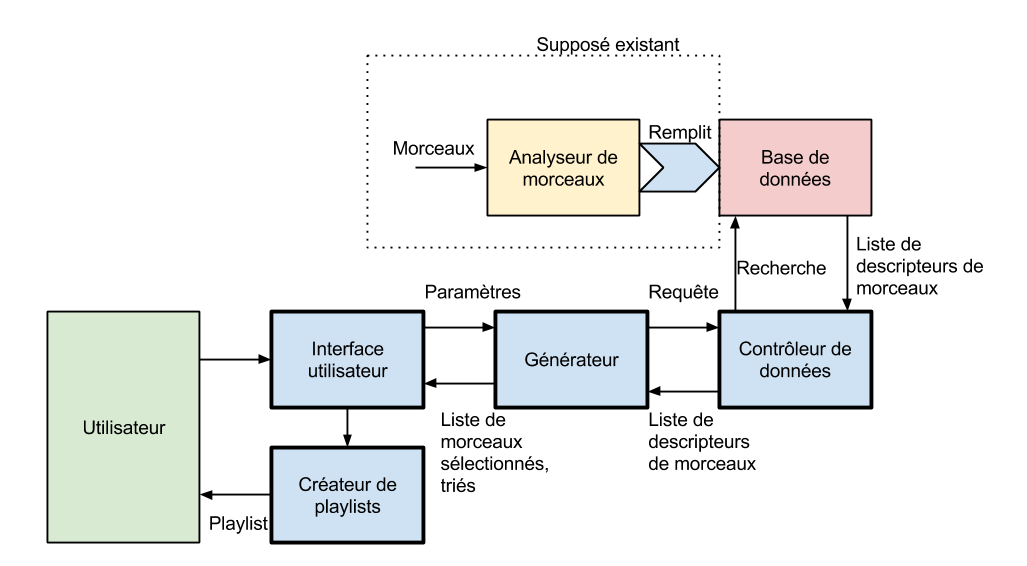
\includegraphics[width=14cm]{modules.png}
\caption{Les 4 modules indispensables au bon fonctionnement du programme et leurs
interactions.}
\end{figure}

\subsection{Ergonomie}
Les interfaces utilisateurs devront être utilisables par un utilisateur
non-avancé, être claires et précises, et éviter de perdre l’utilisateur. Les
termes employés sur cette interface devront être écrit dans un vocabulaire
compréhensible de tous.

\newpage

\section{Contraintes}
\label{sec:contraintes}

\subsection{Délais}
Le programme se soit d’être livré pour la date du mardi 8 avril 2014.

\subsection{Autres contraintes}
Nous ne disposons pas d’analyseur de morceaux, et en créer un ne fait pas partie
de notre sujet. Nous devons donc utiliser nous-même une base de données déjà
existante afin de travailler dessus. Nous avons donc choisi d’utiliser la Million
Song Dataset (http://labrosa.ee.columbia.edu/millionsong/) qui contient toutes
les informations dont nous avons besoin. Nous la convertirons en base de données
SQL pour améliorer le temps de récupération des données.
    
Cette base de données pèse 500Go, la conversion doublera la place nécessaire pour
stocker nos bases de données. Bien que nous travaillerons sur un échantillon
restreint au départ, nous devrons disposer d’un espace de travail d’au moins 1
téraoctet, le CREMI nous fournit cet espace de travail.

\newpage

\section{Prototypes}
\label{sec:proto}

\subsection{Interface utilisateur}
    
L'idée de notre interface graphique est de permettre à un utilisateur non aguérri
de faire fonctionner notre programme sans avoir de grandes connaissances en
informatique musicale. C'est pourquoi nous avons choisi de réaliser une interface
graphique simple et au vocabulaire accessible. Par exemple, l'energie du morceau
sera représentée par un curseur pouvant varier de «~léger~» à «~puissant~», sans
proposer à l'utilisateur de choisir une valeur numérique précise, qui ne
représenterait rien à ses yeux.
    
Les différents paramètres d'entrée sont ainsi organisés de façon à partir du plus
basique au plus complèxe, en regroupant les paramètres dits contextuels (artiste,
genre etc.) en haut et les desripteurs audio en dessous (rythme, énergie, etc.).

Enfin nous proposons d'inclure des checkboxs afin que l'utilisateur puisse
choisir quels paramètres il veut ou non prendre en compte, et ainsi lui laisser
la possibilité de choisir le degré de spécification de la playlist.
    
\begin{figure}[!h]
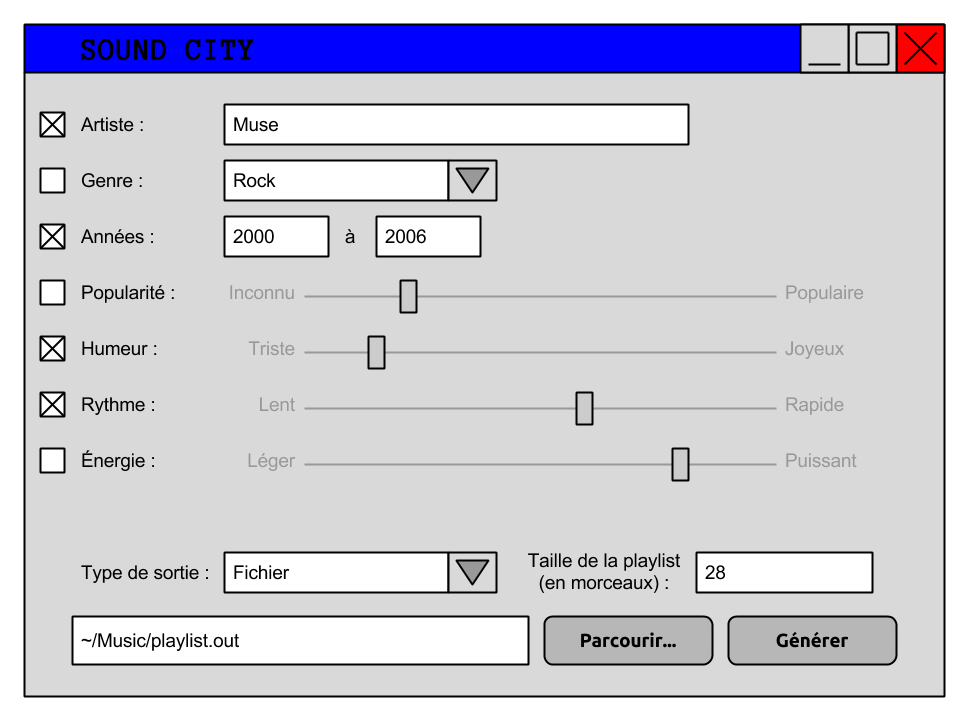
\includegraphics[width=14cm]{interface_utilisateur.png}
\caption{Absence de sorties disponibles à l'initialisation}
\end{figure}

\subsection{Base de données}

La base de données que nous utiliserons sera une conversion en base SQL de la
Million Song Database dont nous extrairons uniquement les valeurs dont nous
avons besoin.
    
\newpage

\section{Scénarios d'utilisation}

\subsection{Initialisation du programme}
    
Lors de l'initialisation du programme, trois cas de figure peuvent être
rencontrés : 

\begin{itemize}
\item L'initialisation se passe correctement et le programme est prêt à être
utilisé.
\item Une erreur est introduide à cause d'un échec de connexion à la base de
données.
\item Une erreur est introduite à cause d'un échec de connexion au module de
sortie.
\end{itemize}

\subsubsection{Initialisation réussie}

Lors du démarrage du programme, l'interface utilisateur va demander au module de
génération de playlists de vérifier la présence d'une base de données accessible.
La rêquete est alors transmise du générateur au module de données qui va
effectuer une connexion avec la base de données.
        
Une fois cette connexion correctement effectuée, le module de données va faire
remonter l'information au générateur qui va à son tour la transmettre à
l'interface utilisateur.

Ensuite l'interface utilisateur s'assure qu'il y a au moins un module de sortie
fonctionnel en récuperant une liste des différentes sorties possibles.

Enfin, l'interface utilisateur s'adapte pour correspondre aux services de sortie
disponibles.
        
\begin{figure}[!h]
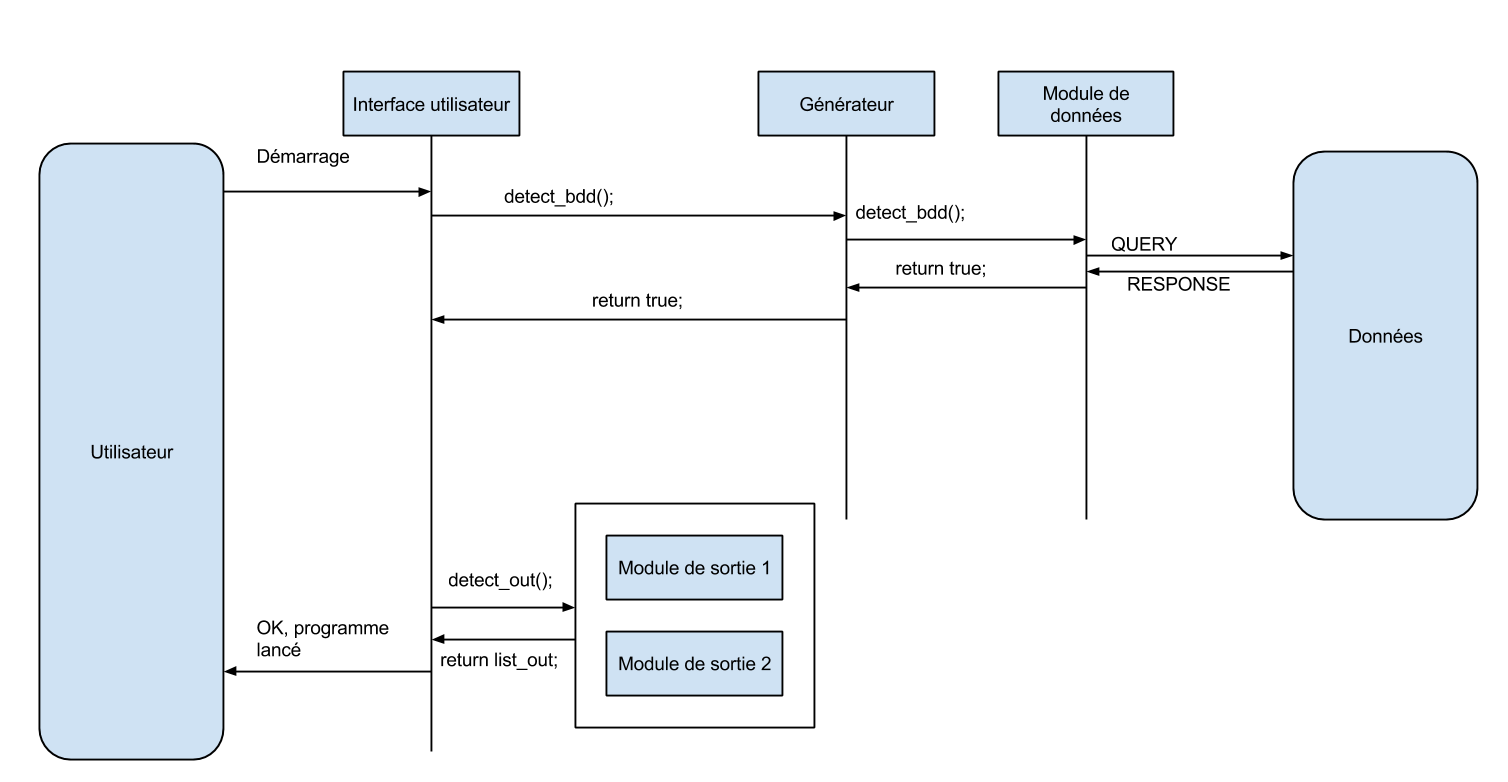
\includegraphics[width=14cm]{demarrage_fonctionnel.png}
\caption{Schéma représentant un prototype d'interface utilisateur}          
\end{figure}
        
\subsubsection{Absence de base de données}
        
Lorsque le module de données tente de se connecter à la base de données, il se
peut que la connexion échoue. Dans ce cas le module de données renvoie au
générateur un message d'erreur qu'il transmet à l'interface utilisateur afin de
l'afficher avant d'arrêter le programme.
        
\begin{figure}[!h]
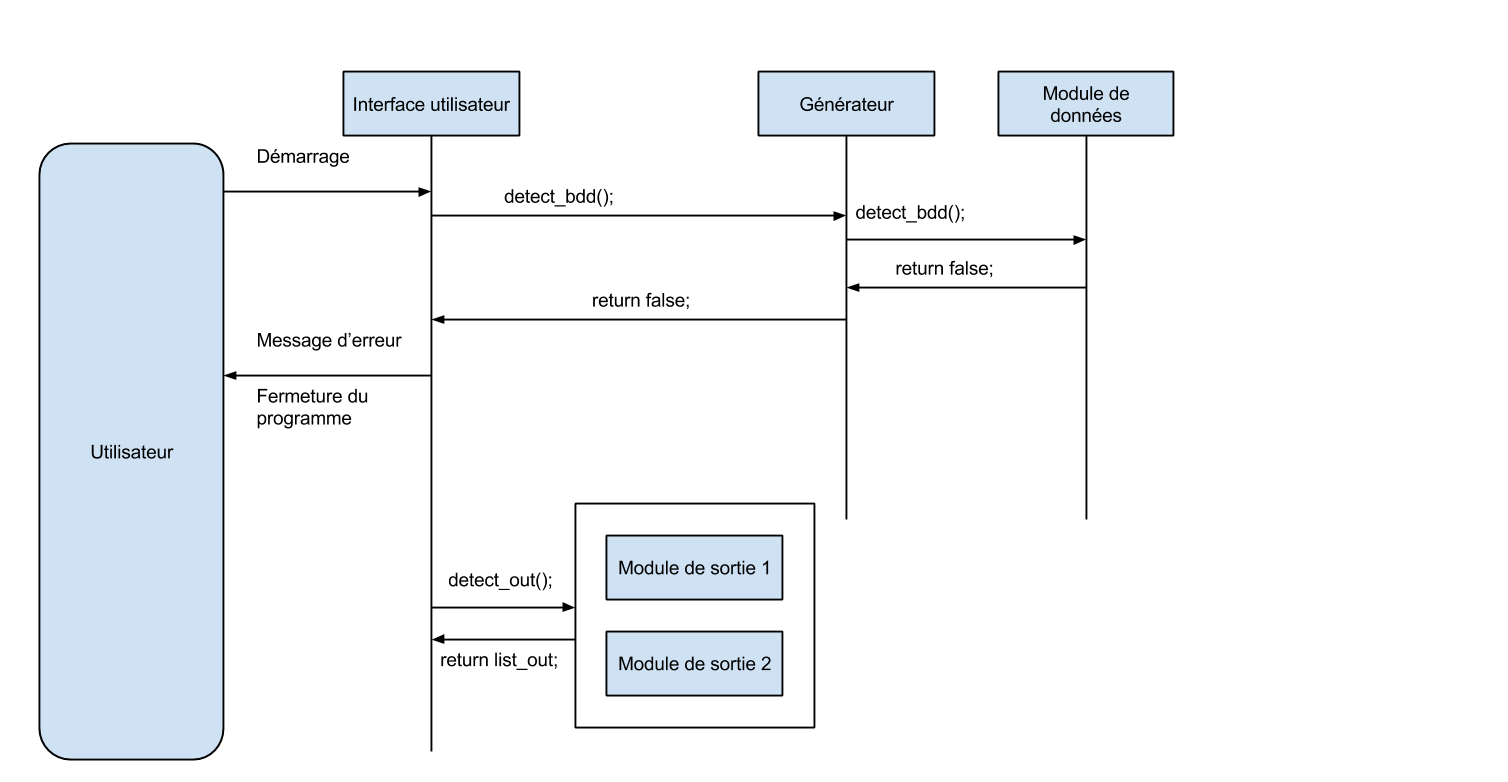
\includegraphics[width=14cm]{demarrage_absence_bdd.png}
\caption{Absence de base de données à l'initialisation}
\end{figure}
        
\subsubsection{Absence de module de sortie}

Dans le cas où l'interface utilisateur effectue correctement une connexion à la
base de données mais n'arrive pas à établir une liste des sorties
disponibles(absence du module de sortie ou aucune sortie disponible), elle doit
afficher un message d'erreur et entraîner l'arrêt du programme.
        
\begin{figure}[!h]
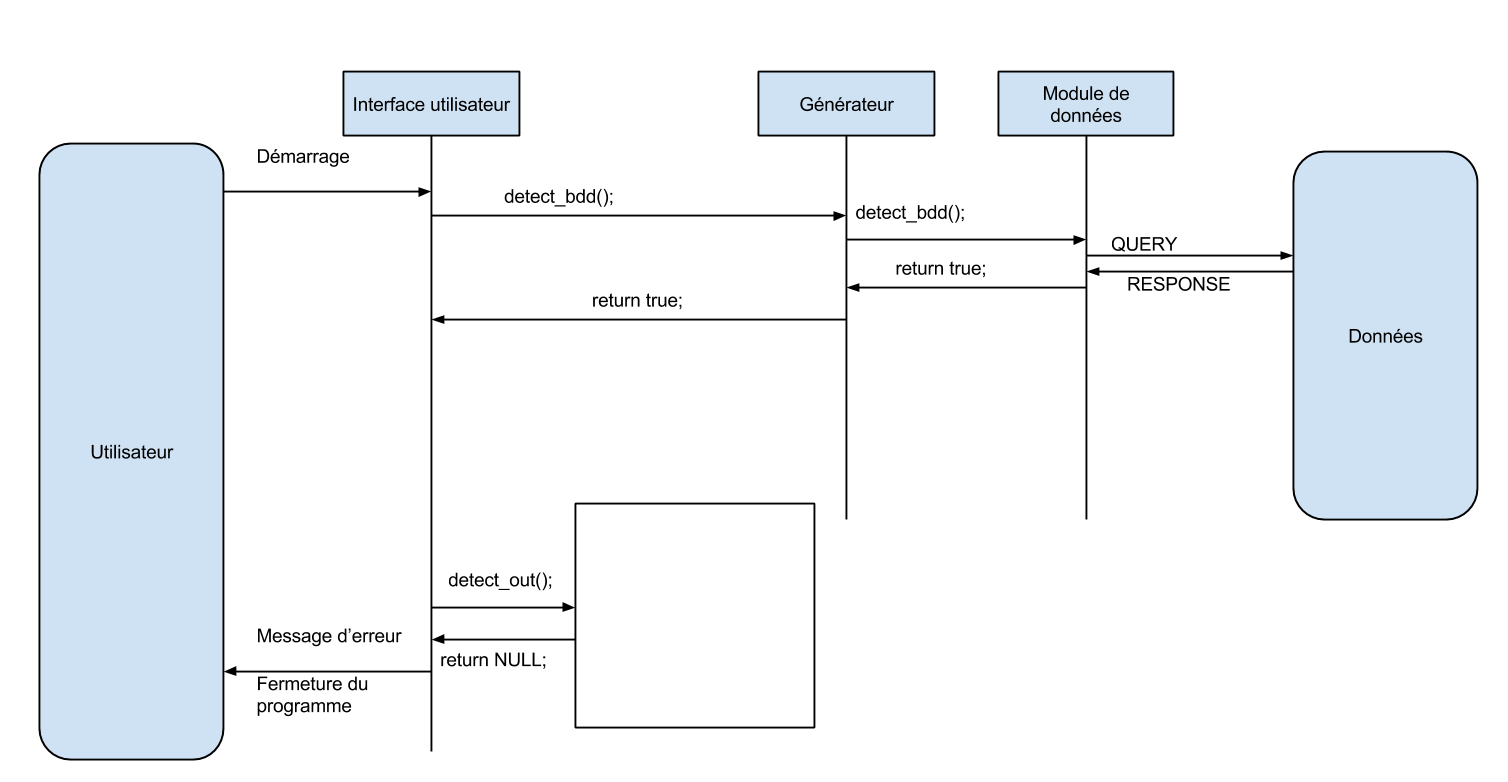
\includegraphics[width=14cm]{demarrage_absence_sortie.png}
\caption{Absence de sorties disponibles à l'initialisation}
\end{figure}
 
\subsection{Génération}

\subsubsection{Génération normale}

\begin{enumerate}
\item L'utilisateur décide de lancer une génération.
\item Le module d'interface utilisateur appelle le module de génération et lui
transmet les paramètres entrées par l'utilisateur.
\item Le module de génération appelle le module de données et lui transmet une
requête de morceaux.
\item Le module de données lance les requêtes SQL à la base de données et
récupère les informations.
\item Les informations rendues au module de générations sont utilsées pour
créer une liste de morceaux.
\item Le module de génération calcule la bonne similarité de la playlist.
\item Le module de génération renvoie la playlist à l'interface utilisateur qui
l'a passe au module de sortie demandée par l'utilisateur.
\item Le module de sortie génére la sortie et la rend directement à
l'utilisateur en passant par l'interface.
\end{enumerate}

\begin{figure}[!h]
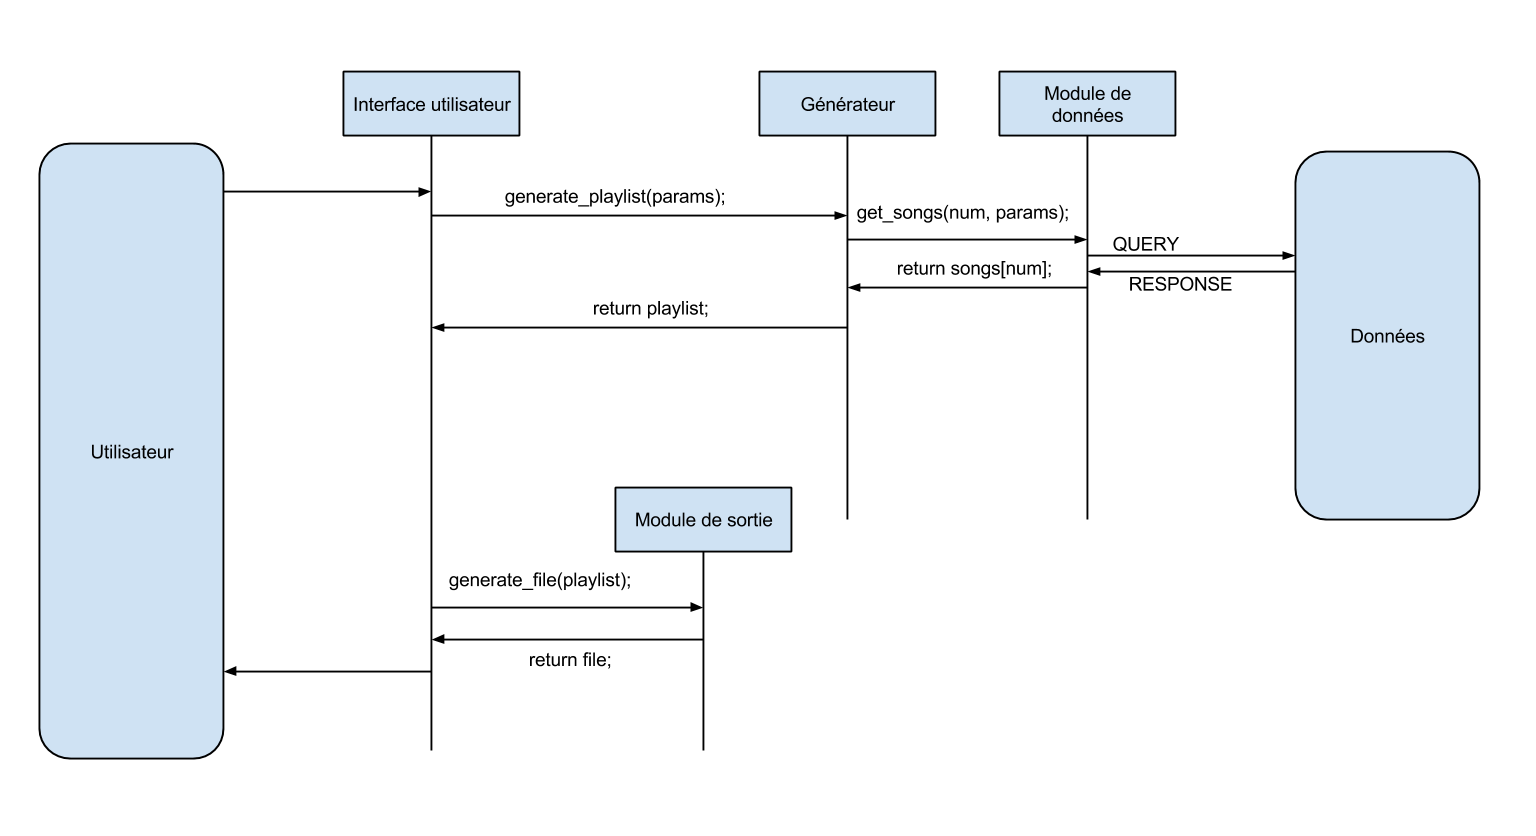
\includegraphics[width=14cm]{generation_fonctionnel.png}
\caption{Génération de playlist réussie}
\end{figure}

\subsubsection{Génération non satisfaisante}

\begin{enumerate}
\item L'utilisateur décide de lancer une génération.
\item Le module d'interface utilisateur appelle le module de génération et lui
transmet les paramètres entrées par l'utilisateur.
\item Le module de génération appelle le module de données et lui transmet une
requête de morceaux.
\item Le module de données lance les requêtes SQL à la base de données et
récupère les informations.
\item Les informations rendues au module de générations sont utilsées pour créer
une liste de morceaux.
\item Le module de génération calcule la bonne similarité de la playlist et
celle ci ne répond pas aux attentes.
\item Le module de génération renvoie la playlist  à l'interface utilisateur qui
demande à l'utilisateur si il veut affiner la recherche ou non.
\item Si oui, on lance une nouvelle génération en gardant la liste générée au
passage précédent (On répète les étapes 3, 4, 5 et 6). Si non, on passe à
l'étape suivante directement.
\item Le module de génération renvoie la playlist à l'interface utilisateur qui
l'a passe au module de sortie demandée par l'utilisateur.
\item Le module de sortie génére la sortie et la rend directement à
l'utilisateur en passant par l'interface.
\end{enumerate}

\begin{figure}[!h]
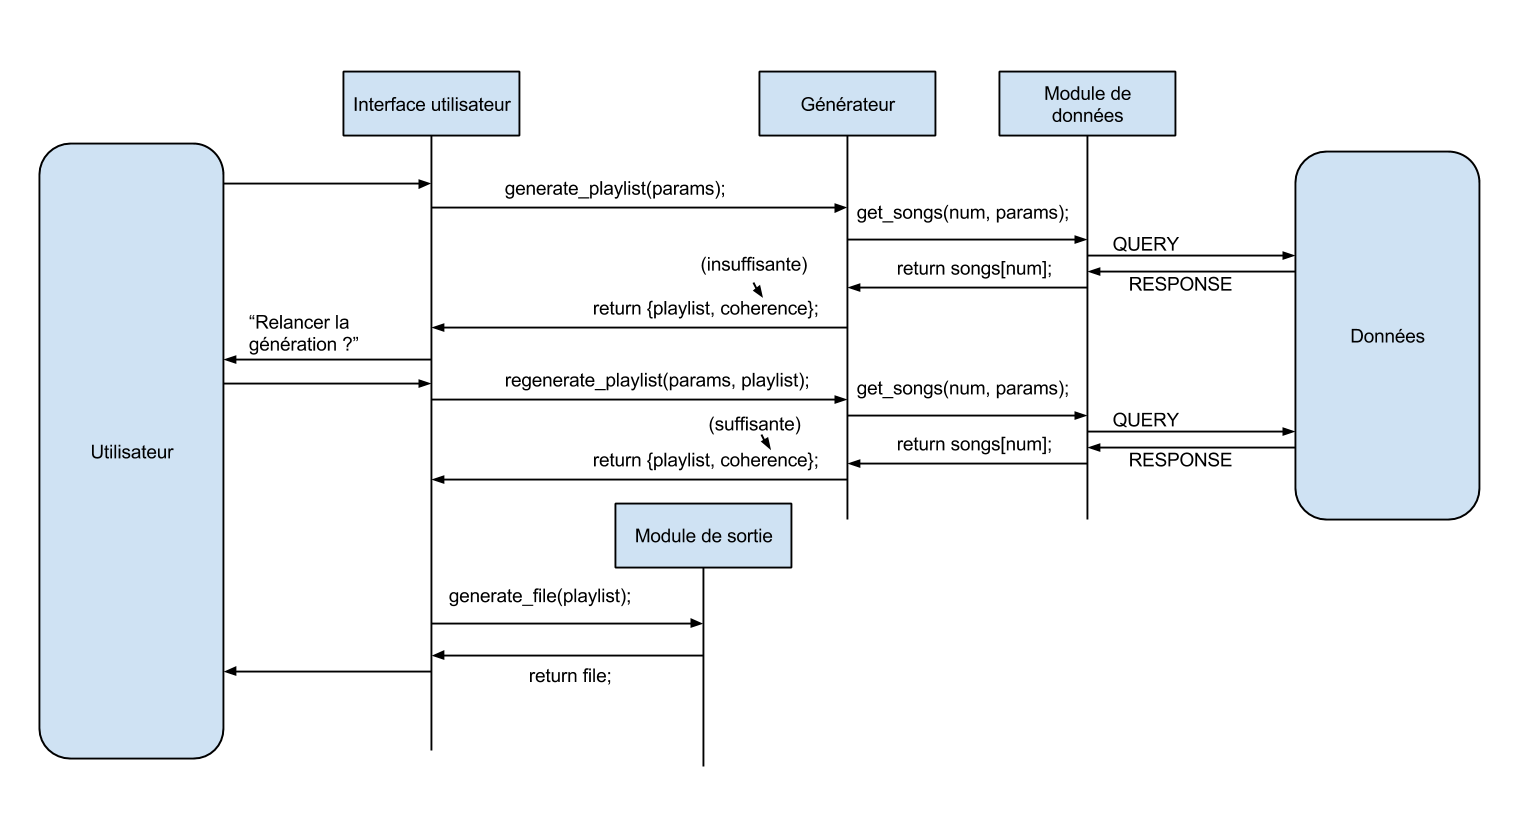
\includegraphics[width=14cm]{generation_decevante.png}
\caption{Génération de playlist non staisfaisante, l'utilisateur relance la génération}
\end{figure}
 

\subsubsection{Génération incomplète}

\begin{enumerate}
\item L'utilisateur décide de lancer une génération.
\item Le module d'interface utilisateur appelle le module de génération et lui
transmet les paramètres entrées par l'utilisateur.
\item Le module de génération appelle le module de données et lui transmet une
requête de morceaux.
\item Le module de données lance les requêtes SQL à la base de données et
récupère les informations, mais n'en récupère pas assez.
\item Les informations rendues au module de générations sont utilsées pour créer
une liste de morceaux.
\item Le module de génération calcule la bonne similarité de la playlist.
\item Le module de génération renvoie la playlist à l'interface utilisateur.
\item L'interface utilisateur avertit l'utilisateur que la playlist estincomplète.
\item L'interface utilisateur passe la playlist au module de sortie demandée
par l'utilisateur.
\item Le module de sortie génére la sortie et la rend directement à
l'utilisateur en passant par l'interface.
\end{enumerate}

\begin{figure}[!h]
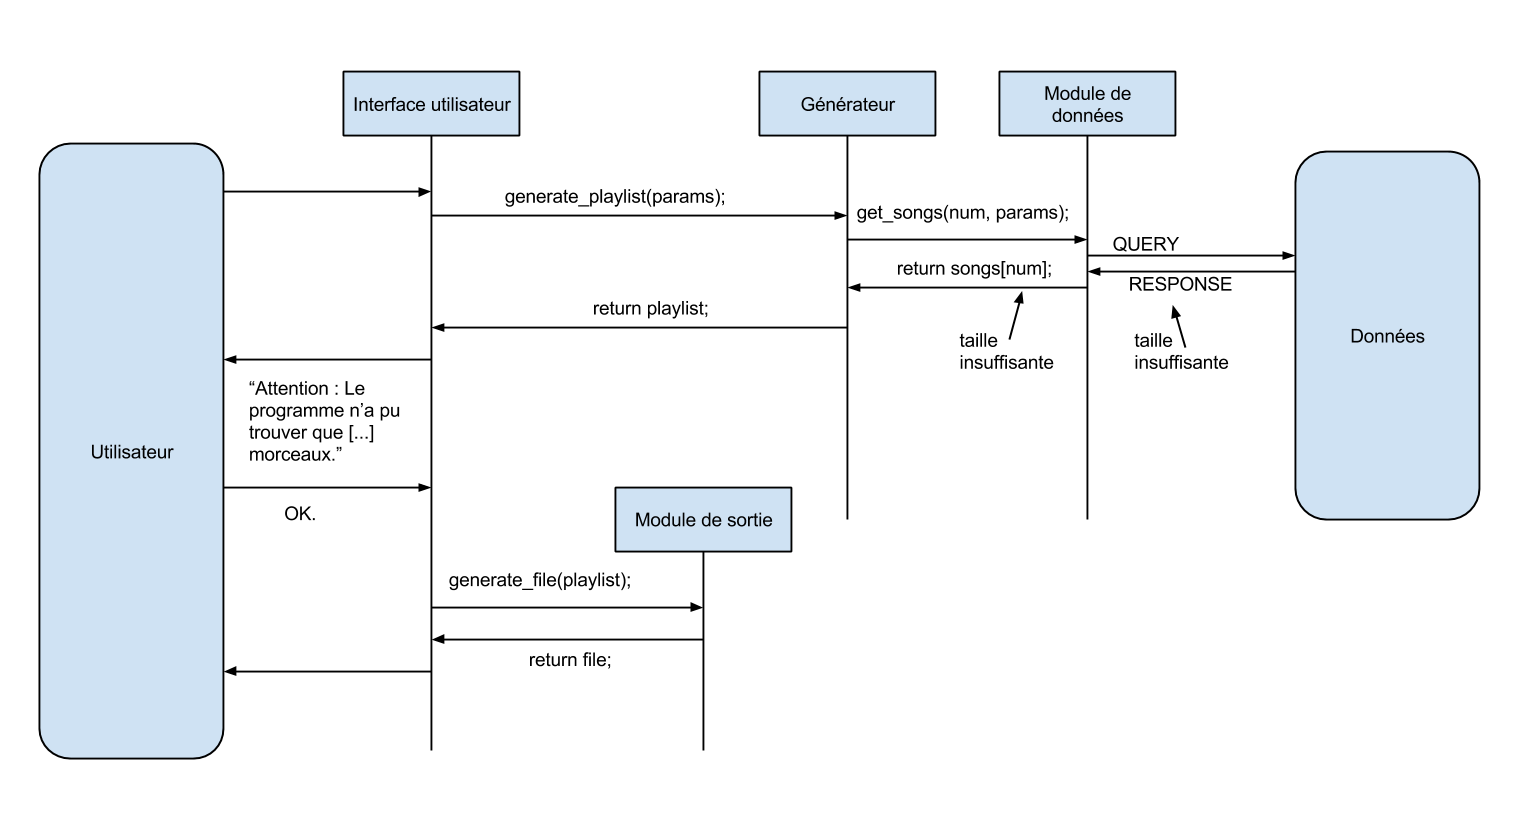
\includegraphics[width=14cm]{generation_incomplete.png}
\caption{Génération terminée mais incomplète, on avertit l'utilisateur}
\end{figure}
 

\subsubsection{Absence de données répondant aux paramètres}

\begin{enumerate}
\item L'utilisateur décide de lancer une génération.
\item Le module d'interface utilisateur appelle le module de génération et lui
transmet les paramètres entrées par l'utilisateur.
\item Le module de génération appelle le module de données et lui transmet une
requête de morceaux.
\item Le module de données lance les requêtes SQL à la base de données et
récupère les informations, mais n'en récupère pas.
\item Le module de génération renvoie une liste vide à l'interface utilisateur.
\item L'interface utilisateur avertit l'utilisateur que la requête ne renvoie
aucune information et qu'aucune playlist ne peut être générée.
\end{enumerate}

\begin{figure}[!h]
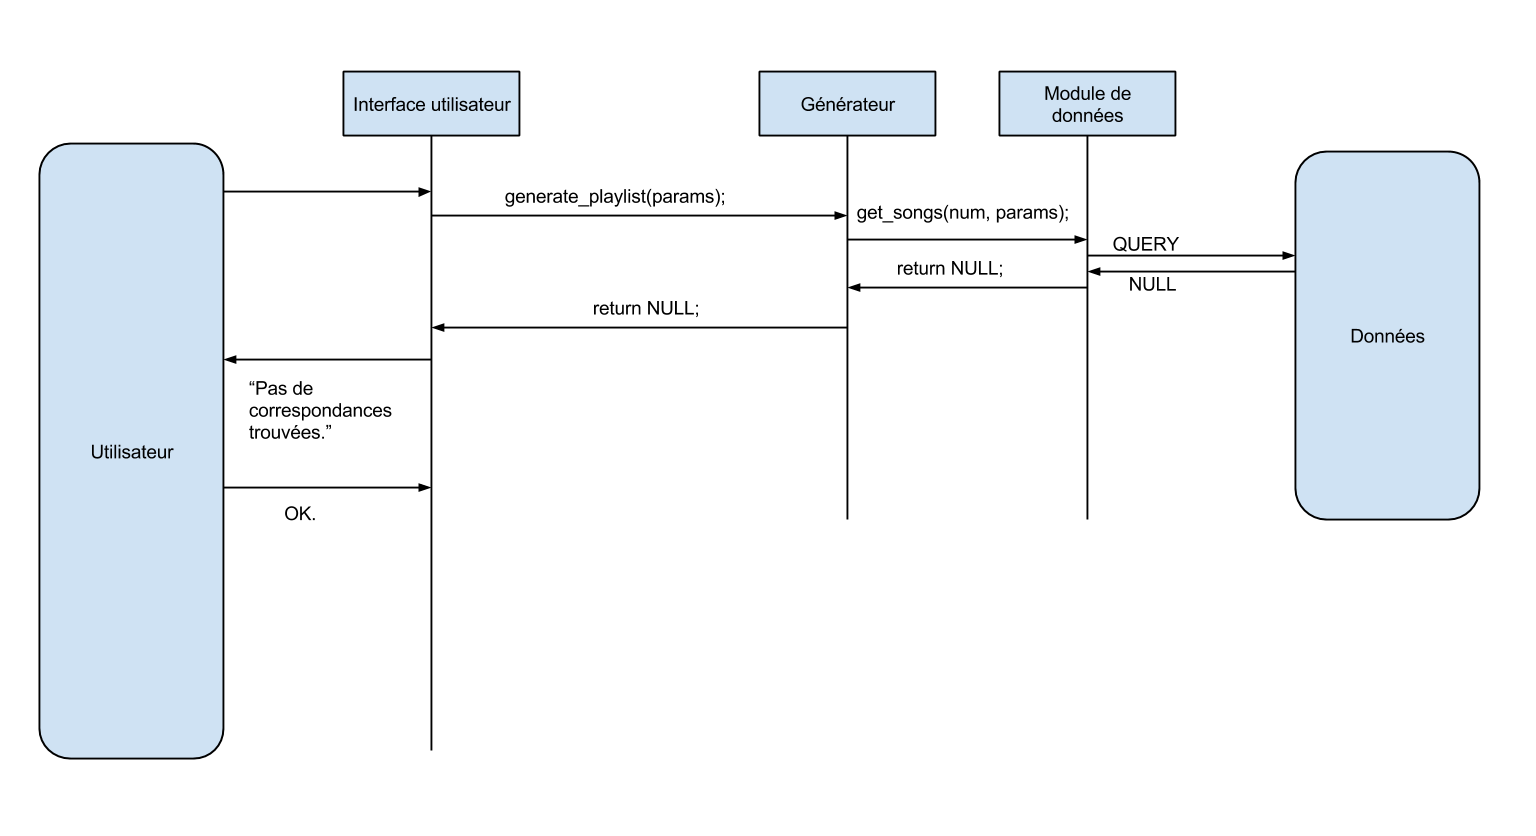
\includegraphics[width=14cm]{generation_nulle.png}
\caption{Génération impossible, il n'y a pas de morceaux correspondants à la requête}
\end{figure}
 
\newpage
\section{Annexes}

\begin{figure}[!h]
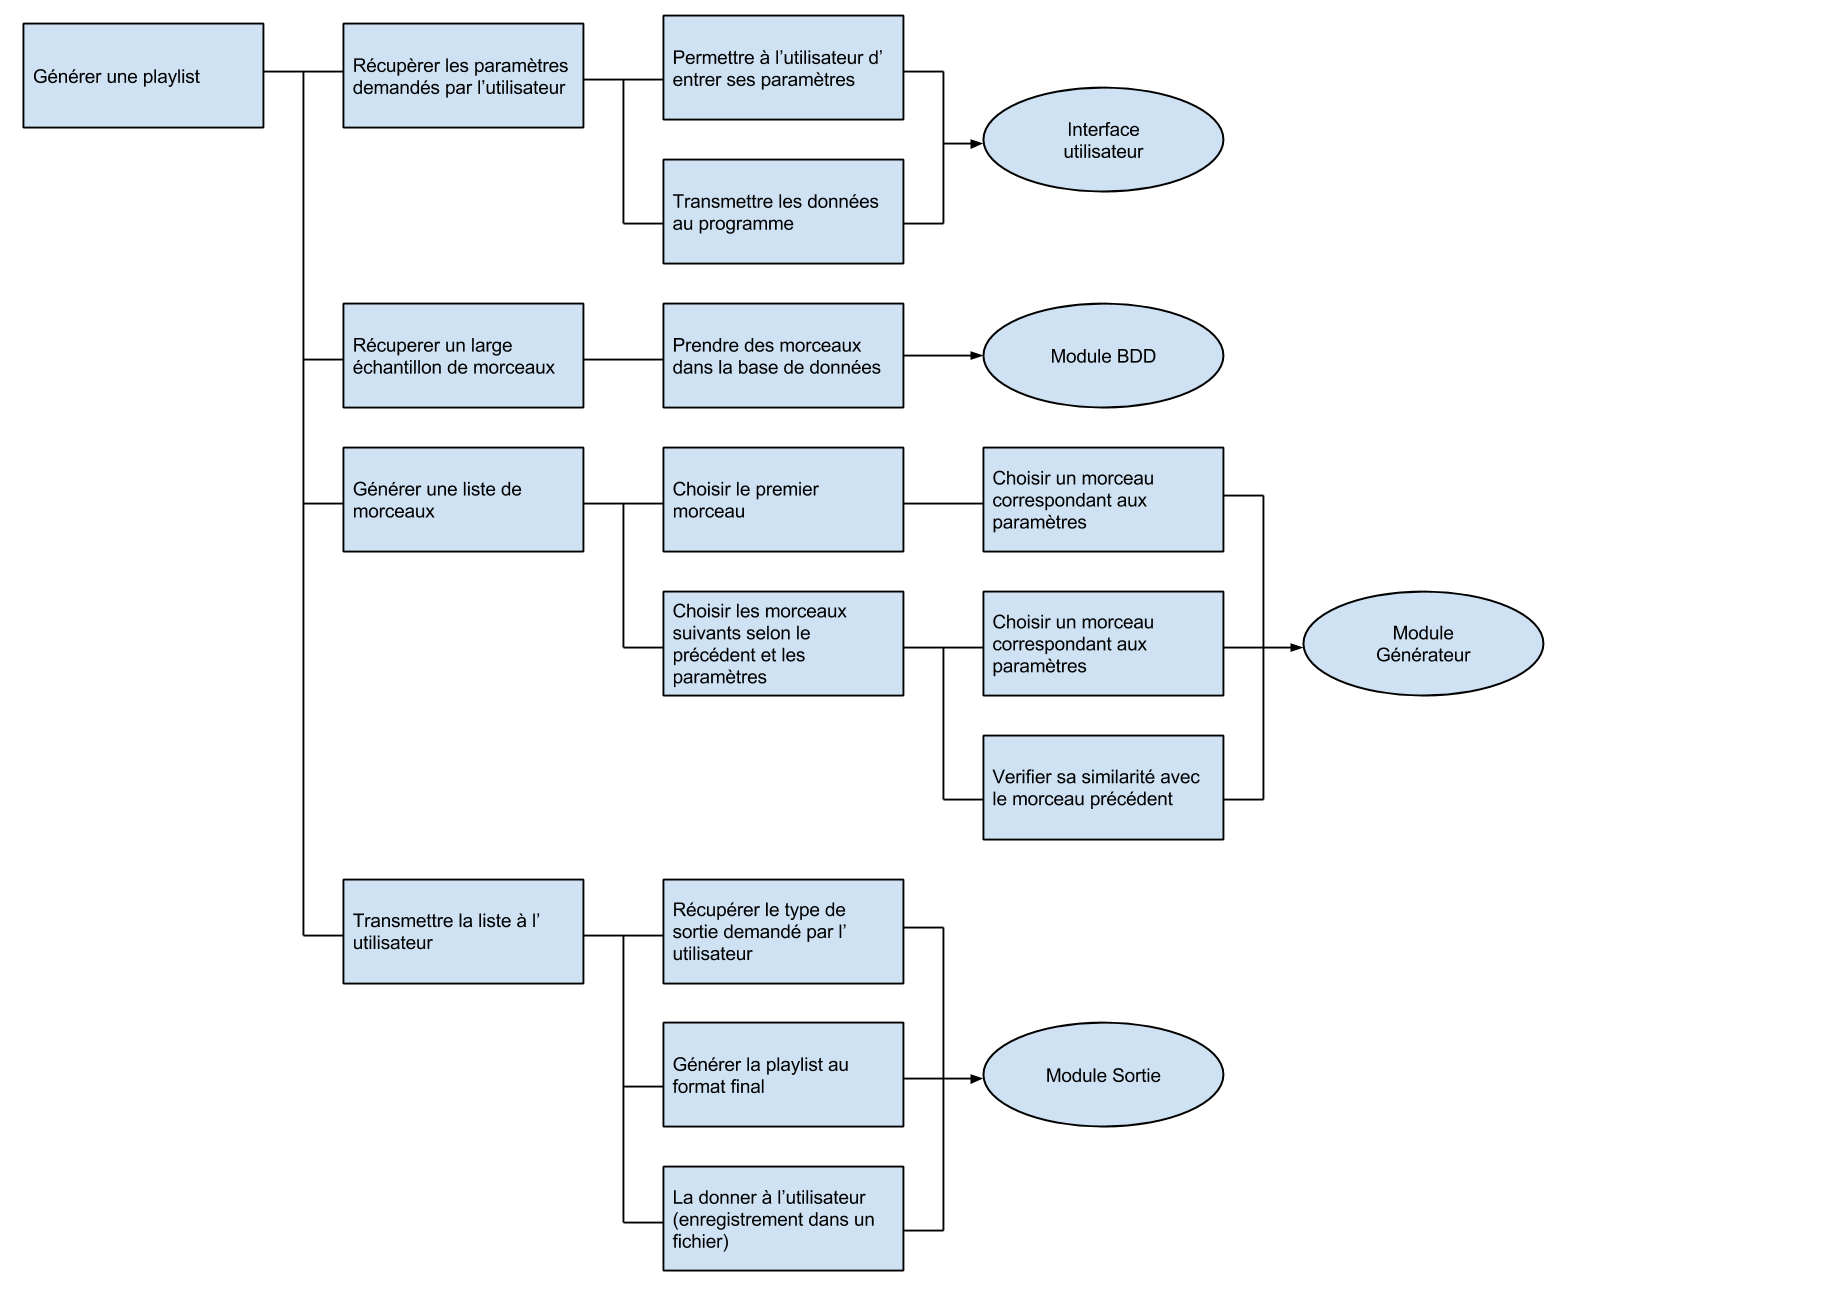
\includegraphics[width=14cm]{fast.png}
\caption{Diagramme FAST illustrant les modules du programme}
\end{figure}

\end{document}